\providecommand{\pmse}[1]{\,{\scriptsize$\pm$#1}}
\section{Experiments}
\label{sec:experiments}

%%AZ.9.12: be more specific, what argument are you testing? Do you just mean the 3 components you modify? just say that.
%%AZ.9.12: looks like we're actually missing this ablation in the experiments. I think it's important to have something that tests each of the 3 modifications to FB (I guess you might only be able to show this as two modifications, since the 3rd is meant to address the first)
%%AZ.9.12: please include a baselines section that explains these baselines and why they were chosen.
%%AZ.9.20: maybe I missed something, what does squared successor approximation mean here?
%%AZ.9.20: why which? it makes it sound like not all the design decisions were necessary. Shouldn't we know which help preserve ordering?
Our experiments test whether FB's least squares approximation can discard rare but control-critical action distinctions, and whether the \name{} preserves those distinctions through normalization and the subsequent policy extraction process introduced in \cref{sec:method}.
We first isolate approximation errors in a didactic MDP with exact SMs, varying feature dimension, examining FB's learned feature span, and ablating \name{}'s components (\cref{sec:exp-didactic}). 
To connect these findings to manipulation, we examine policy failures alongside critic predictions of how actions change future cube occupancies (\cref{fig:failure}).
We then evaluate downstream performance on OGBench~\citep{park-iclr25b}, MetaWorld~\citep{mclean-neurips25a}, and ManiSkill~\citep{tao-rss25a}, and assess performance beyond manipulation using ExoRL datasets~\cite{yarats-arxiv22a} on Deepmind Control Suite (DMC) (\cref{sec:exp-manipulation}).

\paragraph{Experimental protocol.}
%%AZ.9.20: do you mean proprioceptive state here? As in not pixel?
All methods operate on proprioceptive states and are trained for $10^6$ gradient steps on the same fixed offline dataset.
We report results over $5$ independent training seeds.
For offline policy learning, we use the actor from \citet{bagatella-iclr26a}, based on Flow Q-Learning~\citep{park-icml25a}.
Success rates are averaged over the final three evaluations, with $20$ episodes per task on OGBench, $50$ on MetaWorld and ManiSkill, and $10$ for evaluations with an inferred task vector (\cref{tab:hparams}).
Full implementation details are given in \cref{app:implementation} of the appendix.

\paragraph{Baselines.}
We compare against two groups of methods.
\begin{inparaenum}
    \item We consider methods that learn reusable representations from the offline dataset: \textbf{FB}~\citep{touati-neurips21a,touati-iclr23b}, our primary baseline, together with \textbf{HILP}~\citep{park-iclr24a} and \textbf{RLDP}~\citep{jajoo-iclr26a} to test whether the manipulation failure is shared by alternative geometric and predictive representations. 
    \item We compare against goal-conditioned offline RL methods: \textbf{GCIQL}~\cite{kostrikov-iclr22a,park-iclr25b}, \textbf{CRL}~\cite{eysenbach-neurips22a}, and \textbf{QRL}~\cite{wang-icml23a}. 
    These methods train directly for goal reaching using hindsight goals sampled from the offline data, and help us examine how well the zero-shot policies compare with methods trained explicitly for goal-reaching control. 
\end{inparaenum}

\subsection{Distinguishing actions at a control bottleneck}
\label{sec:exp-didactic}
%%AZ.9.12: this is the env where you should also conduct the ablations on Density-FB.

We use the nine-state MDP in \cref{fig:didactic-mdp}, with a fixed continuation policy and exact successor measures. 
At state $2$, the actions enter differently rewarded branches before reaching a shared tail, giving a true action-value gap of $1$.
We vary the feature dimension and report ten runs per setting; \Cref{app:bottleneck-family} gives the setup and additional policy settings.

\paragraph{Do the critics distinguish the two actions?}
With four features, FB assigns the two bottleneck actions identical values, whereas \name{} recovers their exact values (\cref{fig:bottleneck-values}).
To examine whether better forward fitting could recover the missing gap, we freeze FB's learned backward features and refit the forward vectors to the exact successor densities by $\rho$-weighted least squares.
The fitted occupancies remain indistinguishable (\cref{fig:bottleneck-lemma}), illustrating \Cref{lem:linear-action-difference}: the learned feature span cannot recover the difference between the two branches.
\Cref{fig:bottleneck-prop} relates \name{}'s KL error to the sufficient preservation threshold of \cref{prop:bottleneck-preservation}.

\begin{figure}[htb]
    \centering
    \begin{subfigure}[b]{0.32\textwidth}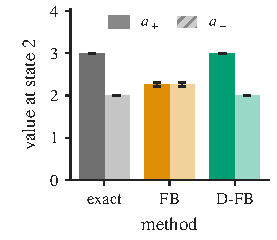
\includegraphics[width=\linewidth]{ICLR/figures/nine_state/fig_61_values.pdf}\caption{}\label{fig:bottleneck-values}\end{subfigure}\hfill
    \begin{subfigure}[b]{0.32\textwidth}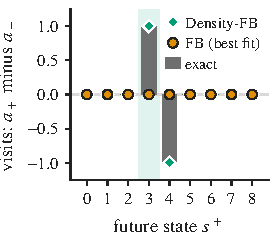
\includegraphics[width=\linewidth]{ICLR/figures/nine_state/fig_61_lemma.pdf}\caption{}\label{fig:bottleneck-lemma}\end{subfigure}\hfill
    \begin{subfigure}[b]{0.32\textwidth}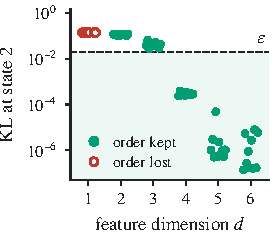
\includegraphics[width=\linewidth]{ICLR/figures/nine_state/fig_61_prop.pdf}\caption{}\label{fig:bottleneck-prop}\end{subfigure}
    \caption{
    \textbf{At the bottleneck of \cref{fig:didactic-mdp}, FB's features erase the action-value difference; \name{} keeps it.}
    \emph{(a)} Predicted and exact action values at the bottleneck with four features (D-FB: \name{}); mean and $95\%$ interval over ten runs.
    \emph{(b)} Differences ($a_+-a_-$) in discounted future visits. Gray bars: exact. Orange: best least-squares fit on FB's frozen features. Green: \name{} at the same dimension.
    \emph{(c)} KL divergence from the exact model to \name{}'s predicted successor distribution at state $2$ (hollow red: $a_-$ ranked above $a_+$). Below the dashed threshold $\varepsilon$ of \cref{prop:bottleneck-preservation} the ordering is guaranteed.
    }
    \label{fig:bottleneck-main}
\end{figure}

\paragraph{Preserving action-value gaps with fewer features.}
Normalizing FB's target leaves recovery near zero through six features, whereas applying a softmax recovers the full gap with four features under either squared error or cross-entropy (\Cref{fig:ablation}).
The softmax parameterization therefore accounts for the capacity advantage in this MDP.
Smoothing the immediate target instead limits recovery to approximately $71\%$; \Cref{app:bottleneck-ablation} outlines the variants.

\begin{figure}[htb]
    \centering
    \begin{minipage}[c]{0.50\textwidth}
        \centering
        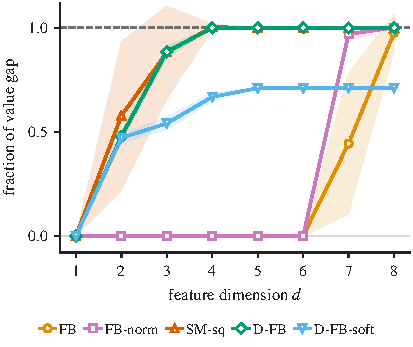
\includegraphics[width=\linewidth]{ICLR/figures/nine_state/fig_61_ablation_main.pdf}
    \end{minipage}\hfill
    \begin{minipage}[c]{0.47\textwidth}
        \captionsetup{justification=raggedright,singlelinecheck=false}
        \caption{
        \textbf{\name{} keeps the action-value difference with fewer features.}
        Predicted value difference at state $2$ divided by the exact one, against the feature dimension; mean and $95\%$ interval over ten TD runs.
        The dashed line is exact recovery.
        The variants are defined in \cref{app:bottleneck-ablation}.
        }
        \label{fig:ablation}
    \end{minipage}
\end{figure}


\paragraph{From tabular bottlenecks to manipulation tasks.}
We next examine where FB fails in manipulation tasks and whether the critic captures how changing an action changes the cube's future in the \texttt{cube-single} from OGBench.
Following \citet{mohan-rlbrew26a}, we classify each evaluation episode as successful or by its first failed stage (\Cref{fig:failure}, Top). 
Most FB failures occur after grasping, while holding or carrying the cube. \name{} has fewer failures at both stages (\cref{fig:failure-where}).
We next examine the corresponding critic predictions by restoring states from each phase and comparing predicted differences between two actions' discounted future cube occupancies with rollout estimates under the critic's continuation policy.
Both methods have near-zero cosine alignment during approach, but \name{} aligns more closely during holding and carrying, with the largest separation during transport (\Cref{fig:failure-align}).

\begin{figure}[t]
    \centering
    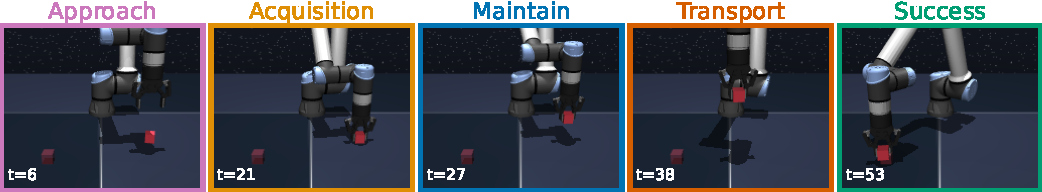
\includegraphics[width=\linewidth]{ICLR/figures/failure/fig_phase_strip.pdf}\\[4pt]
    \begin{minipage}[b]{0.50\linewidth}
        \centering
        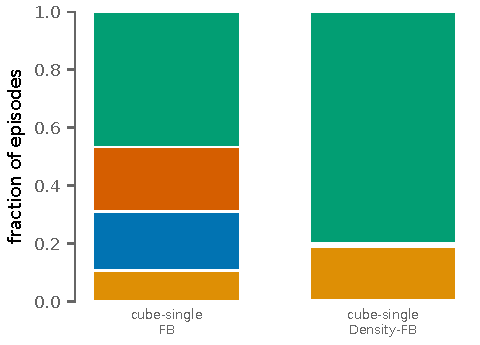
\includegraphics[width=\linewidth]{ICLR/figures/failure/fig_failure_where.pdf}
        \phantomsubcaption\label{fig:failure-where}
    \end{minipage}\hfill
    \begin{minipage}[b]{0.46\linewidth}
        \centering
        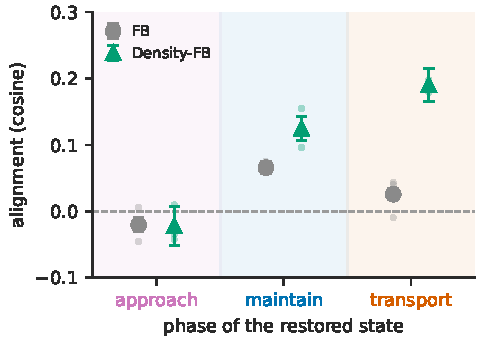
\includegraphics[width=\linewidth]{ICLR/figures/gap_preservation/fig_alignment_by_phase_main.pdf}
        \phantomsubcaption\label{fig:failure-align}
    \end{minipage}
    % \ben{It'd be great to illustrate the phases in a picture / video clip.}
   \caption{
        \textbf{Cube manipulation failures and critic alignment.}
        Top: the stages in one successful \name{} episode on \texttt{cube-single} (translucent cube: goal).
        (a) First failed stage:
        \textcolor[HTML]{CC78BC}{approach} (reach),
        \textcolor[HTML]{DE8F05}{acquisition} (grasp),
        \textcolor[HTML]{0173B2}{maintain} (hold), or
        \textcolor[HTML]{D55E00}{transport} (carry to goal);
        \textcolor[HTML]{029E73}{success} denotes completion.
        (b) Cosine similarity between predicted and rollout-estimated
        action differences in discounted future cube visits;
        zero indicates no directional alignment.
        Large markers and error bars show mean $\pm$ SE over evaluated
        states; small markers show the three seed means.
    }
    \label{fig:failure}
\end{figure}


\begin{table}[t]
    \centering
    \caption{\textbf{Performance across benchmarks.} Results are mean $\pm$ SE over five seeds. Benchmark rows average tasks, with propagated SEs. \textbf{Bold} marks the best mean and others within its SE. $\Delta$ reports \name{}'s relative improvement over the best baseline (\%), colored from red ($\le -25\%$) through gray to green ($\ge +25\%$); ``--'' denotes inapplicable goal-conditioned baselines.}
    \label{tab:benchmarks}
    % Tighten + scale to fit \textwidth
    \setlength{\tabcolsep}{3pt}
    \renewcommand{\arraystretch}{1.05}
    \scriptsize
    \resizebox{\textwidth}{!}{%
    \begin{tabular}{lrrrrrrrr}
    \toprule
    Task/Domain                             & FB                        & HILP              & RLDP                      & GCIQL                     & CRL               & QRL                       & \name{}                   & \shortstack[r]{$\Delta$ next best} \\
    \midrule
    \textit{OGBench (success rate, \%)}    & 18.7\pmse{1.3} & 38.3\pmse{2.0} & 14.0\pmse{0.7} & 53.0\pmse{1.0} & 16.0\pmse{0.4} & 3.7\pmse{0.2} & \textbf{78.4}\pmse{0.9} & \textcolor[RGB]{0,150,40}{($+$47.9\%)} \\
    \midrule
    \texttt{cube-single}                   & 45.1\pmse{2.9} & 64.4\pmse{4.8} & 27.5\pmse{1.2} & 68.0\pmse{2.1} & 19.0\pmse{0.7} & 5.0\pmse{0.4} & \textbf{93.1}\pmse{0.6} & \textcolor[RGB]{0,150,40}{($+$36.9\%)} \\
    \texttt{cube-double}                   & 1.7\pmse{1.1} & 9.2\pmse{1.7} & 2.8\pmse{0.4} & 40.0\pmse{1.8} & 10.0\pmse{0.7} & 1.0\pmse{0.0} & \textbf{69.5}\pmse{1.2} & \textcolor[RGB]{0,150,40}{($+$73.8\%)} \\
    \texttt{scene}                         & 9.3\pmse{2.2} & 41.3\pmse{3.1} & 11.6\pmse{1.7} & 51.0\pmse{1.4} & 19.0\pmse{0.7} & 5.0\pmse{0.4} & \textbf{72.5}\pmse{2.3} & \textcolor[RGB]{0,150,40}{($+$42.2\%)} \\
    \midrule
    \textit{MetaWorld (success rate, \%)}  & 52.5\pmse{5.9} & 33.1\pmse{3.5} & 39.7\pmse{5.3} & 10.0\pmse{3.3} & 16.9\pmse{2.7} & \textbf{87.7}\pmse{0.8} & 85.2\pmse{2.8} & \textcolor[RGB]{113,91,91}{($-$2.9\%)} \\
    \midrule
    \texttt{push}                          & 29.6\pmse{3.4} & 17.2\pmse{3.8} & 57.6\pmse{1.7} & 4.0\pmse{1.5} & 18.4\pmse{2.6} & 80.8\pmse{1.1} & \textbf{91.2}\pmse{1.9} & \textcolor[RGB]{49,126,69}{($+$12.9\%)} \\
    \texttt{bin-picking}                   & 62.4\pmse{17.4} & 49.2\pmse{9.1} & 19.6\pmse{15.4} & 0.0\pmse{0.0} & 0.0\pmse{0.0} & \textbf{98.0}\pmse{1.0} & 92.4\pmse{2.4} & \textcolor[RGB]{125,82,82}{($-$5.7\%)} \\
    \texttt{box-close}                     & 65.6\pmse{1.8} & 32.8\pmse{3.4} & 42.0\pmse{3.8} & 26.0\pmse{9.7} & 32.4\pmse{7.8} & \textbf{84.4}\pmse{1.8} & 72.0\pmse{7.7} & \textcolor[RGB]{165,53,53}{($-$14.7\%)} \\
    \midrule
    \textit{ManiSkill (success rate, \%)}  & 63.3\pmse{1.7} & 44.4\pmse{2.4} & 56.0\pmse{1.6} & 36.5\pmse{1.0} & 13.4\pmse{1.8} & 65.8\pmse{0.9} & \textbf{77.3}\pmse{1.0} & \textcolor[RGB]{30,135,58}{($+$17.5\%)} \\
    \midrule
    \texttt{push-cube}                     & 88.7\pmse{3.4} & 49.2\pmse{6.3} & 40.8\pmse{3.5} & 68.4\pmse{1.9} & 29.6\pmse{6.9} & \textbf{96.4}\pmse{0.4} & \textbf{97.2}\pmse{1.2} & \textcolor[RGB]{97,102,98}{($+$0.8\%)} \\
    \texttt{pick-cube}                     & 4.4\pmse{0.4} & 6.4\pmse{1.3} & \textbf{39.6}\pmse{2.9} & 2.8\pmse{0.4} & 4.4\pmse{0.7} & 7.2\pmse{1.3} & \textbf{40.8}\pmse{3.2} & \textcolor[RGB]{88,106,93}{($+$3.0\%)} \\
    \texttt{stack-cube}                    & \textbf{70.4}\pmse{3.0} & 56.8\pmse{5.7} & 57.2\pmse{3.7} & 28.0\pmse{3.4} & 2.4\pmse{1.0} & \textbf{67.6}\pmse{1.5} & \textbf{70.8}\pmse{3.3} & \textcolor[RGB]{98,101,99}{($+$0.6\%)} \\
    \texttt{poke-cube}                     & 90.0\pmse{1.9} & 51.2\pmse{5.9} & 58.4\pmse{5.3} & 73.6\pmse{1.7} & 10.8\pmse{1.2} & \textbf{92.0}\pmse{2.3} & \textbf{92.8}\pmse{1.6} & \textcolor[RGB]{97,102,98}{($+$0.9\%)} \\
    \texttt{lift-peg}                      & 63.2\pmse{6.8} & 58.4\pmse{6.0} & \textbf{84.0}\pmse{1.7} & 9.6\pmse{2.6} & 20.0\pmse{5.3} & 66.0\pmse{3.4} & \textbf{84.7}\pmse{1.1} & \textcolor[RGB]{97,102,98}{($+$0.8\%)} \\
    \bottomrule
    \end{tabular}%
    }
\end{table}



\subsection{Performance across benchmarks}
\label{sec:exp-manipulation}

We next evaluate \name{} on 11 manipulation tasks from OGBench, MetaWorld, and ManiSkill, and locomotion tasks in DMC (\cref{tab:benchmarks}).
Dataset details are provided in \cref{app:data-mw-ms}.
\name{} achieves higher mean success than FB on every manipulation task, with average gains of $59.7$, $32.7$, and $14.0$ percentage points on OGBench, MetaWorld, and ManiSkill, respectively. It also exceeds HILP and RLDP on all 11 tasks. Against the goal-conditioned baselines, \name{} achieves the highest mean success on nine tasks, including all three OGBench and all five ManiSkill tasks.
QRL has higher mean success on \texttt{bin-picking} and \texttt{box-close}, and on the MetaWorld average.
\name{} can condition its policy either on a goal state, trained on hindsight goals, or on a task vector inferred from reward samples, trained on a mixture of goal-derived and random task vectors (\cref{app:z-sampling}); both use the same successor model and objective.
We report the version that performs best on each benchmark: goal conditioning on OGBench, and inferred task vectors on MetaWorld, ManiSkill, and ExoRL.
With inferred task vectors, as for FB, HILP, and RLDP, \name{} reaches 82.9\pmse{1.8}, 31.7\pmse{1.4}, and 54.0\pmse{1.6} on \texttt{cube-single}, \texttt{cube-double}, and \texttt{scene}, still above every successor-representation baseline on all three tasks.

\paragraph{Beyond manipulation.}
We also evaluate \name{} on the ExoRL RND datasets (\cref{tab:exorl}).
\name{} attains the highest mean return ($700.5$ vs. $648.2$ for FB), leading on quadruped and point-mass, while FB remains stronger on walker ($-7.6\%$) and cheetah ($-19.7\%$). 
This split is consistent with our analysis: the DMC tasks are dense-reward locomotion problems without interaction bottlenecks, so the failure mode Density-FB targets is largely absent there, and changing the objective brings no systematic advantage.


\begin{table}[t]
    \centering
    \caption{\textbf{ExoRL (DMC returns).} Results are mean $\pm$ SE over five seeds. \textbf{Bold} marks the best mean and others within its SE. $\Delta$ reports \name{}'s relative improvement over the next-best baseline (\%).}
    \label{tab:exorl}
    \renewcommand{\arraystretch}{1.0}
    \tiny

    {\setlength{\tabcolsep}{1.5pt}% tighter columns so it doesn't overflow
    \resizebox{0.90\textwidth}{!}{%
    \begin{tabular}{lrrrrr}
        \toprule
        Task/Domain                             & FB                        & HILP              & RLDP                      & \name{}                   & \shortstack[r]{$\Delta$ next best} \\
        \midrule
        \textit{ExoRL (DMC returns)}           & 648.2\pmse{2.6} & 620.1\pmse{4.5} & 610.2\pmse{7.2} & \textbf{700.5}\pmse{10.3} & \textcolor[RGB]{68,116,81}{($+$8.1\%)} \\
        \midrule
        \texttt{walker}                        & \textbf{811.5}\pmse{2.6} & 796.4\pmse{3.4} & 723.9\pmse{8.2} & 750.2\pmse{13.3} & \textcolor[RGB]{133,76,76}{($-$7.6\%)} \\
        \texttt{quadruped}                     & 595.6\pmse{4.1} & 694.8\pmse{4.9} & 665.0\pmse{6.2} & \textbf{760.5}\pmse{9.1} & \textcolor[RGB]{62,119,77}{($+$9.5\%)} \\
        \texttt{point-mass}                    & 513.0\pmse{8.9} & 371.0\pmse{16.6} & 476.3\pmse{17.6} & \textbf{751.5}\pmse{33.1} & \textcolor[RGB]{0,150,40}{($+$46.5\%)} \\
        \texttt{cheetah}                       & \textbf{672.7}\pmse{2.2} & 618.3\pmse{2.6} & 575.6\pmse{20.1} & 539.9\pmse{18.8} & \textcolor[RGB]{187,37,37}{($-$19.7\%)} \\
        \bottomrule
    \end{tabular}%
    }% end resizebox
    }% end local tabcolsep group
\end{table}


\section{Conclusion}
We studied how SM approximations can erase action-value differences at control bottlenecks. 
Our analysis characterizes this failure under least-squares fitting and establishes sufficient accuracy conditions for preserving action ordering. 
Motivated by these findings, \name{} learns normalized future-state distributions from bilinear scores using a categorical Bellman objective, then evaluates actions by averaging rewards under those distributions.
Across eleven manipulation tasks \name{} outperforms FB on every task. 
Together, these findings emphasize that reusable occupancy predictions must retain the consequences of action choices to support precise control.